\documentclass{article}
\usepackage[final]{neurips_2020}

\usepackage[utf8]{inputenc}
\usepackage{ctex}
\usepackage[T1]{fontenc}    % use 8-bit T1 fonts
\usepackage{hyperref}       % hyperlinks
\usepackage{url}            % simple URL typesetting
\usepackage{booktabs}       % professional-quality tables
\usepackage{amsfonts}       % blackboard math symbols
\usepackage{amsmath}
\usepackage{nicefrac}       % compact symbols for 1/2, etc.
\usepackage{microtype}      % microtypography
\usepackage{indentfirst}
\usepackage{listings}
\usepackage{graphicx}
\usepackage{graphics}
\usepackage{float}
\usepackage{diagbox}
\usepackage[dvipsnames]{xcolor}
\lstset{
    language=Python, % 设置语言
    basicstyle=\ttfamily, % 设置字体族
    breaklines=true, % 自动换行
    keywordstyle=\bfseries\color{NavyBlue}, % 设置关键字为粗体,颜色为 NavyBlue
    morekeywords={}, % 设置更多的关键字,用逗号分隔
    emph={self}, % 指定强调词,如果有多个,用逗号隔开
    emphstyle=\bfseries\color{Rhodamine}, % 强调词样式设置
    commentstyle=\itshape\color{black!50!white}, % 设置注释样式,斜体,浅灰色
    stringstyle=\bfseries\color{PineGreen!90!black}, % 设置字符串样式
    columns=flexible,
    numbers=left, % 显示行号在左边
    numbersep=2em, % 设置行号的具体位置
    numberstyle=\footnotesize, % 缩小行号
    frame=single, % 边框
    framesep=1em, % 设置代码与边框的距离
    showstringspaces=false
}
\setlength{\parindent}{2em}

\title{中山大学计算机院本科生实验报告\\
    (2023学年春季学期)
}

\begin{document}
\maketitle
课程名称:编译原理 \qquad\qquad\qquad\qquad\qquad\qquad
批改人:
\begin{table*}[h]
    \centering
    \begin{tabular}{|c|c|c|c|} \hline
        实验    & LAB1-后缀表达式Postfix                   & 专业(方向) & 计算机科学与技术 计科一班 \\ \hline
        学号    & 21307099                           & 姓名     & 李英骏           \\\hline
        Email & \texttt{liyj323@mail2.sysu.edu.cn} & 完成日期   & \today        \\\hline
    \end{tabular}
\end{table*}
\tableofcontents

\newpage
\section{静态成员与非静态成员}
这是一个单线程程序,并且在整个程序中只存在一个Paser对象,
理论上,是否将lookahead声明为static对于程序的正确性没有任何影响.实验结果记录如下:\\
\textbf{声明为static时,运行./testcase.bat:}
\begin{figure}[H]
    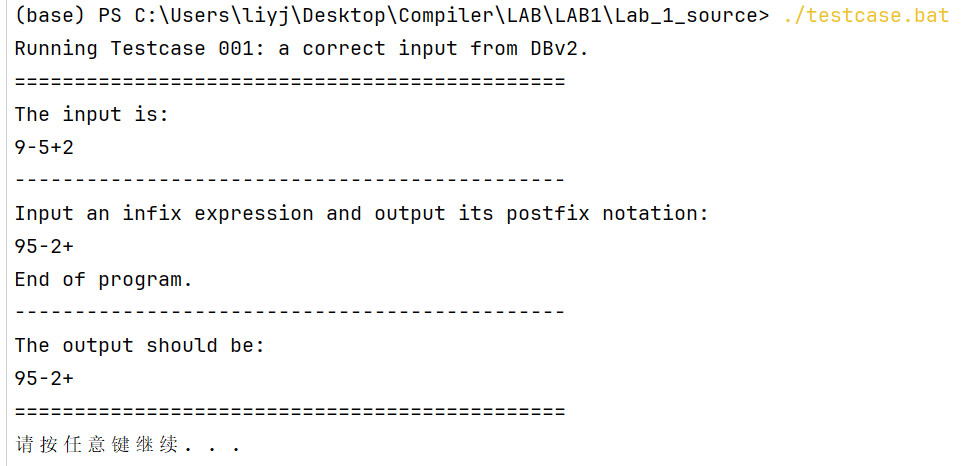
\includegraphics[width=0.65\textwidth]{element/1.png}
    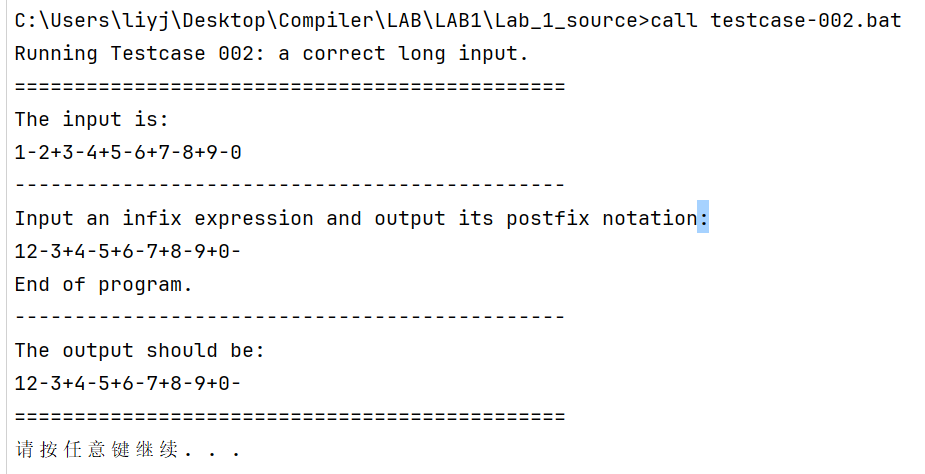
\includegraphics[width=0.65\textwidth]{element/2.png}
    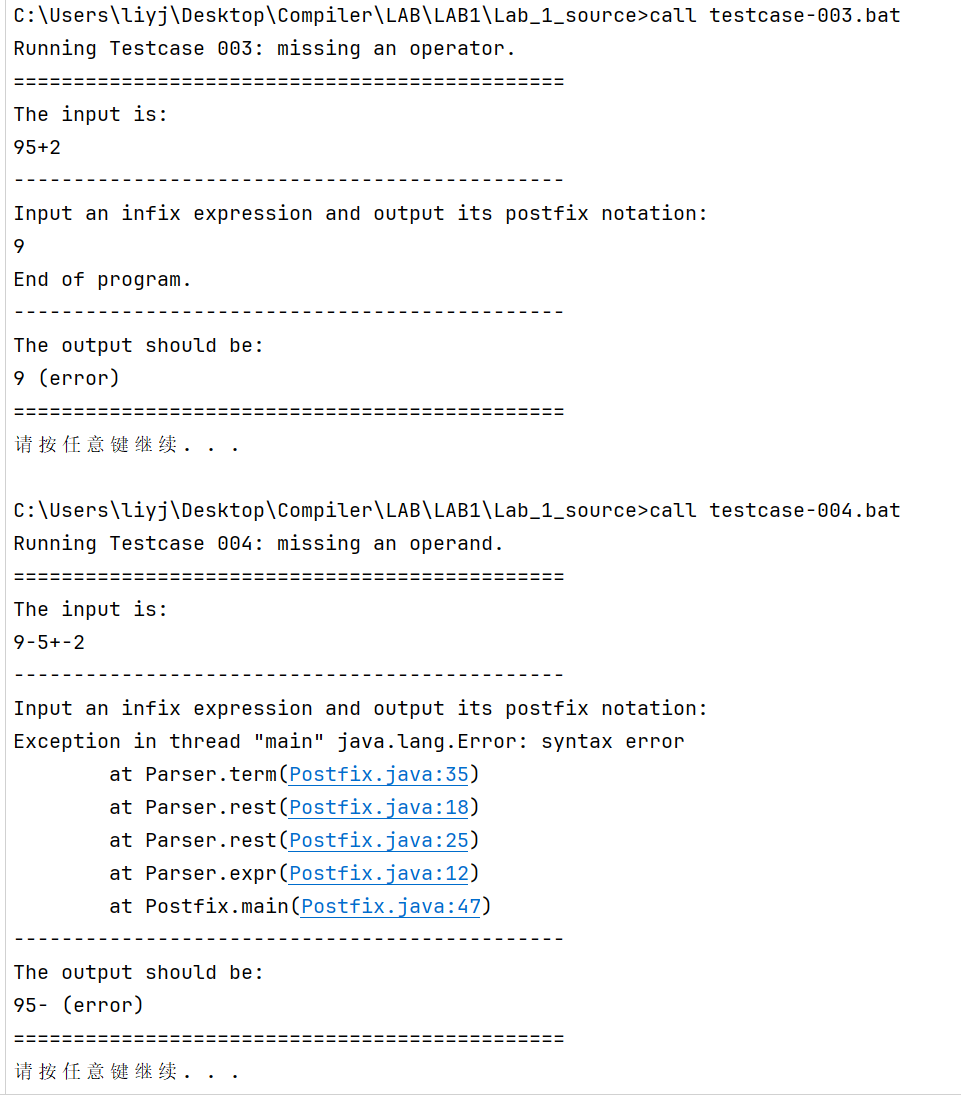
\includegraphics[width=0.65\textwidth]{element/3.png}
    \caption{static}
\end{figure}
\newpage
\noindent
\textbf{去掉static时,运行./testcase.bat:}
\begin{figure}[H]
    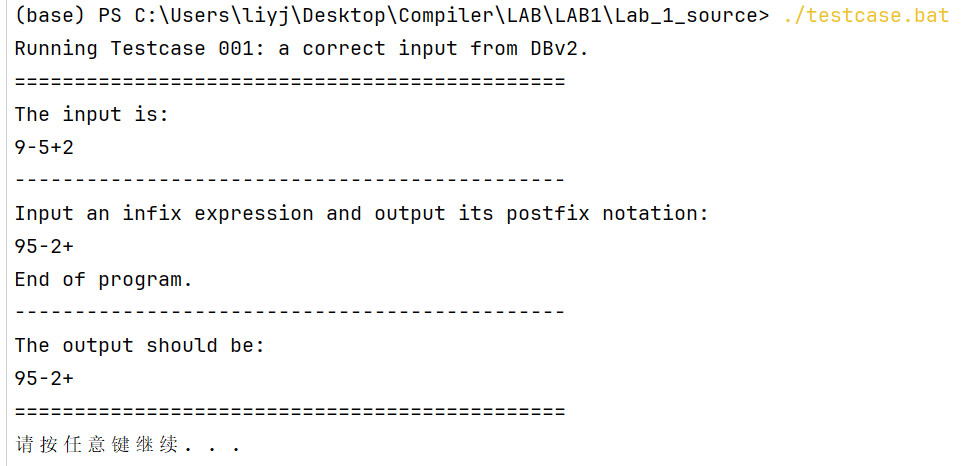
\includegraphics[width=0.65\textwidth]{element/1.png}
    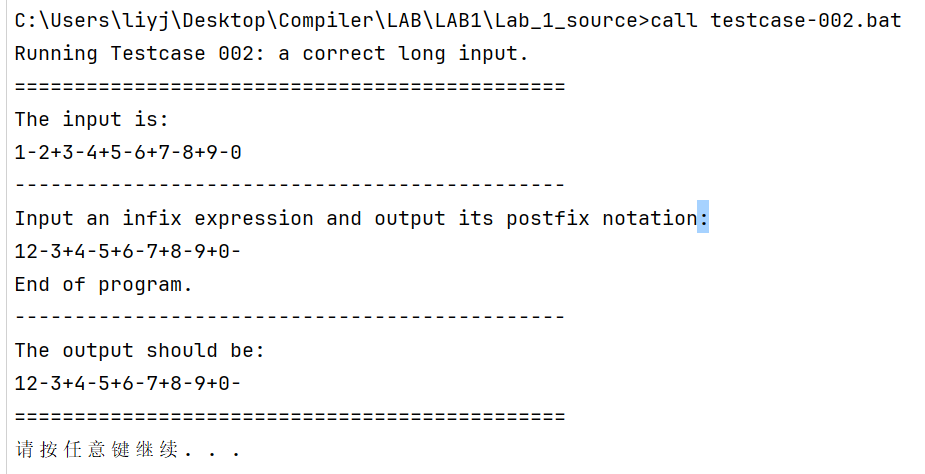
\includegraphics[width=0.65\textwidth]{element/2.png}
    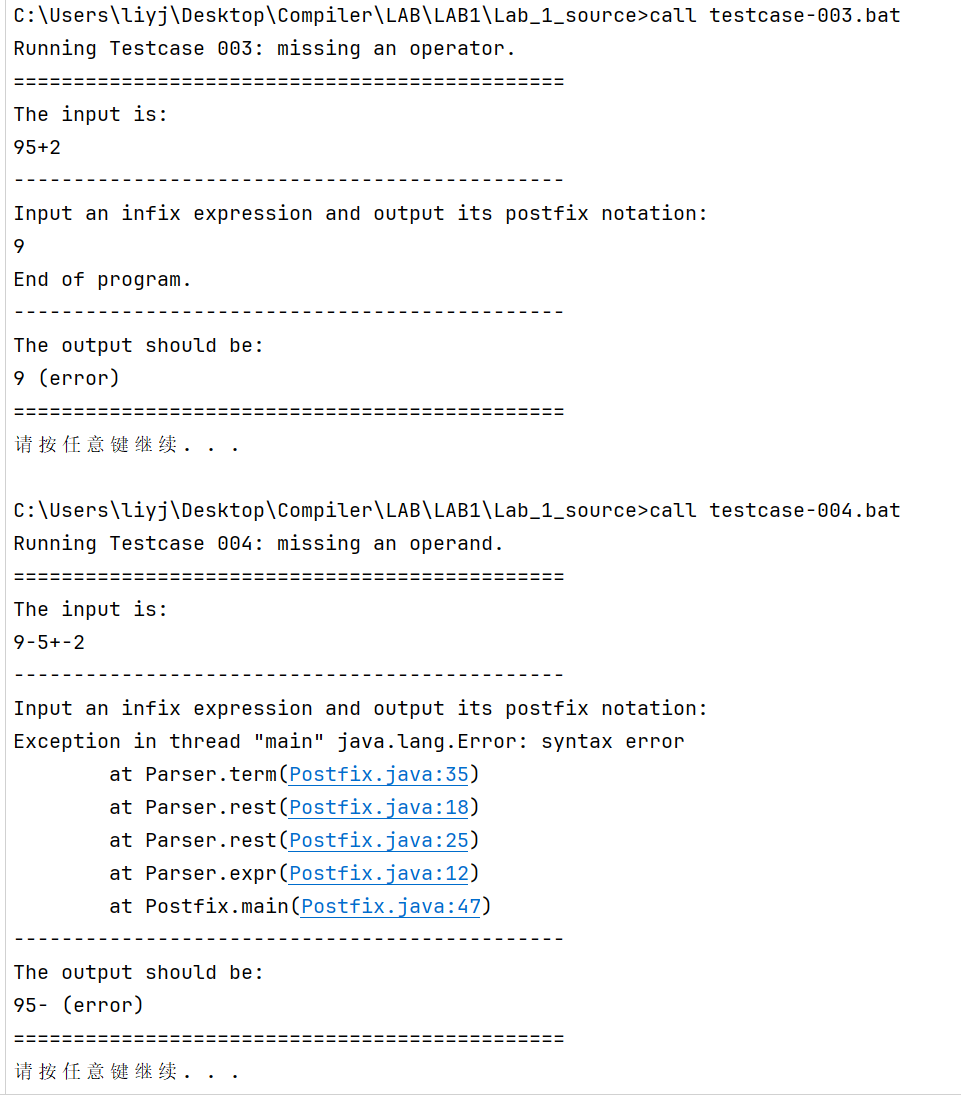
\includegraphics[width=0.65\textwidth]{element/3.png}
    \caption{non\ static}
\end{figure}
可以看到没有任何区别. 我认为声明为\textcolor{red}{非static}更合适,因为
\begin{enumerate}
    \item 在绝大多数需求中,都不会遇到需要多个paser实例解析同一个字符流的情形.
    \item 在单paser实例的应用程序中,是否声明为static影响不大.但static显然会影响代码的扩展性和复用性.
    \item 在可能的多实例或多线程中,lookahead设置为static会导致错误或竞态等线程安全问题.
\end{enumerate}
\newpage
\section{比较消除尾递归前后程序的性能}
消除尾递归如图:
\begin{figure}[H]
    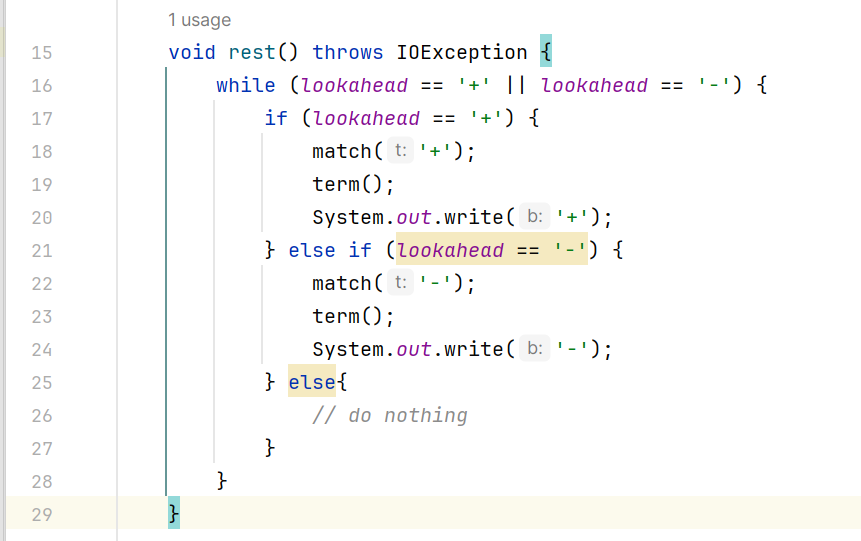
\includegraphics[width=\textwidth]{element/4.png}
    \caption{loop version}
\end{figure}
我们使用如下脚本生成测试数据
\begin{figure}[H]
    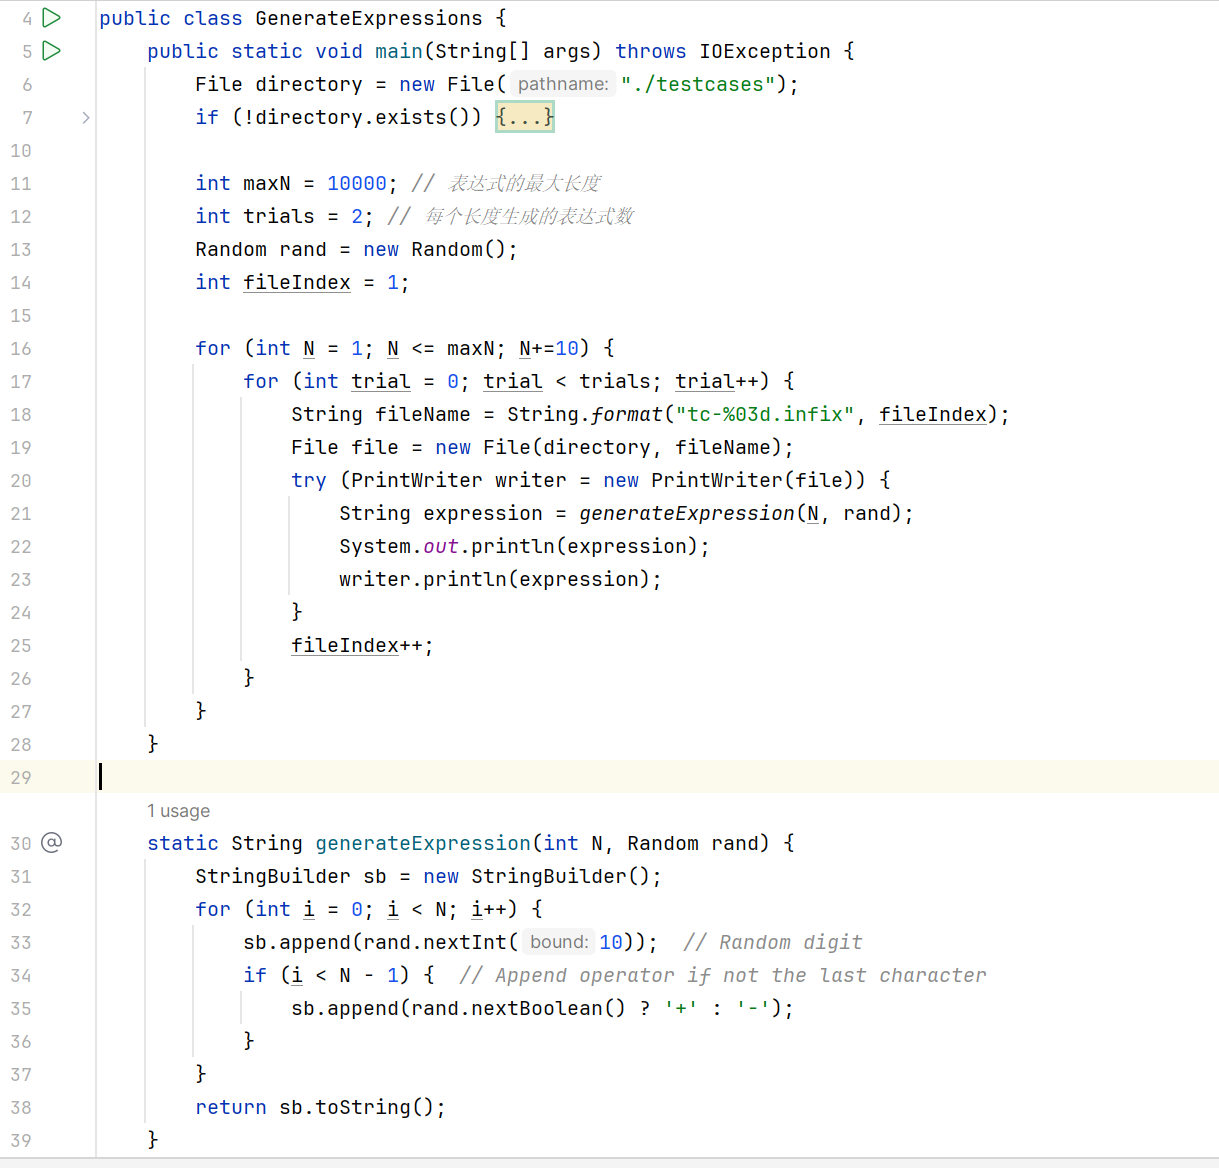
\includegraphics[width=\textwidth]{element/6.png}
    \caption{loop version}
\end{figure}
如图:
\begin{figure}[H]
    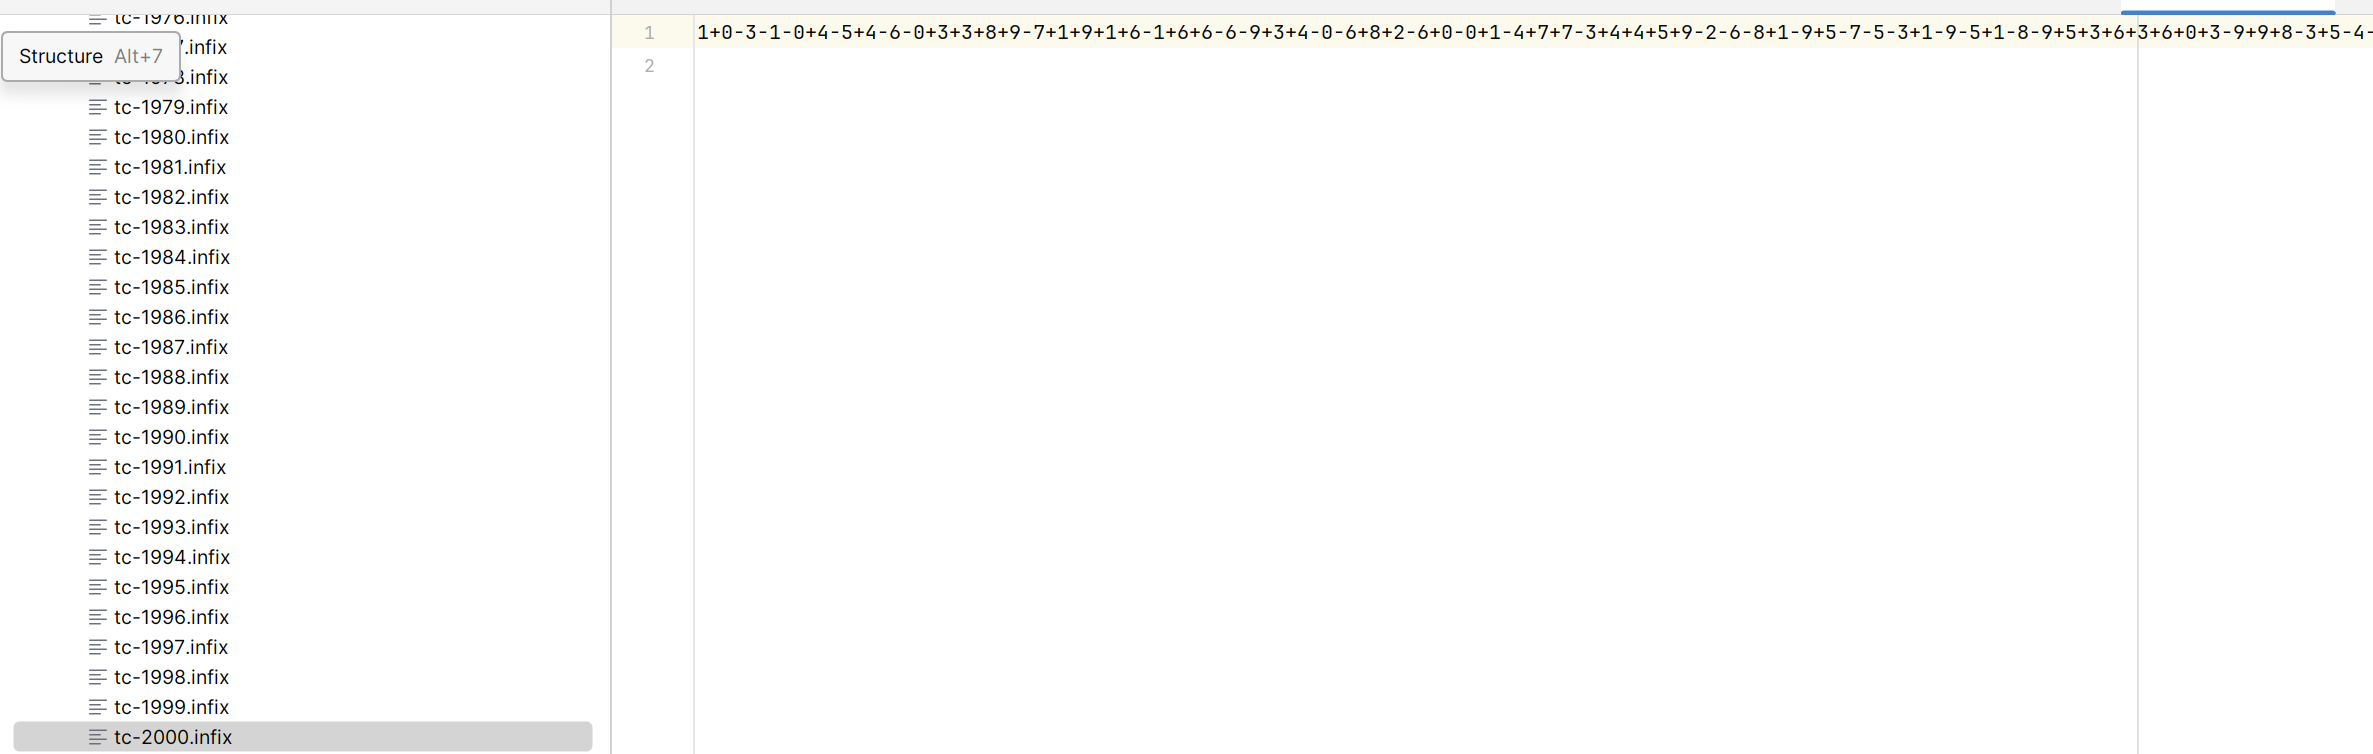
\includegraphics[width=\textwidth]{element/7.png}
    \caption{loop version}
\end{figure}
\begin{figure}[H]
    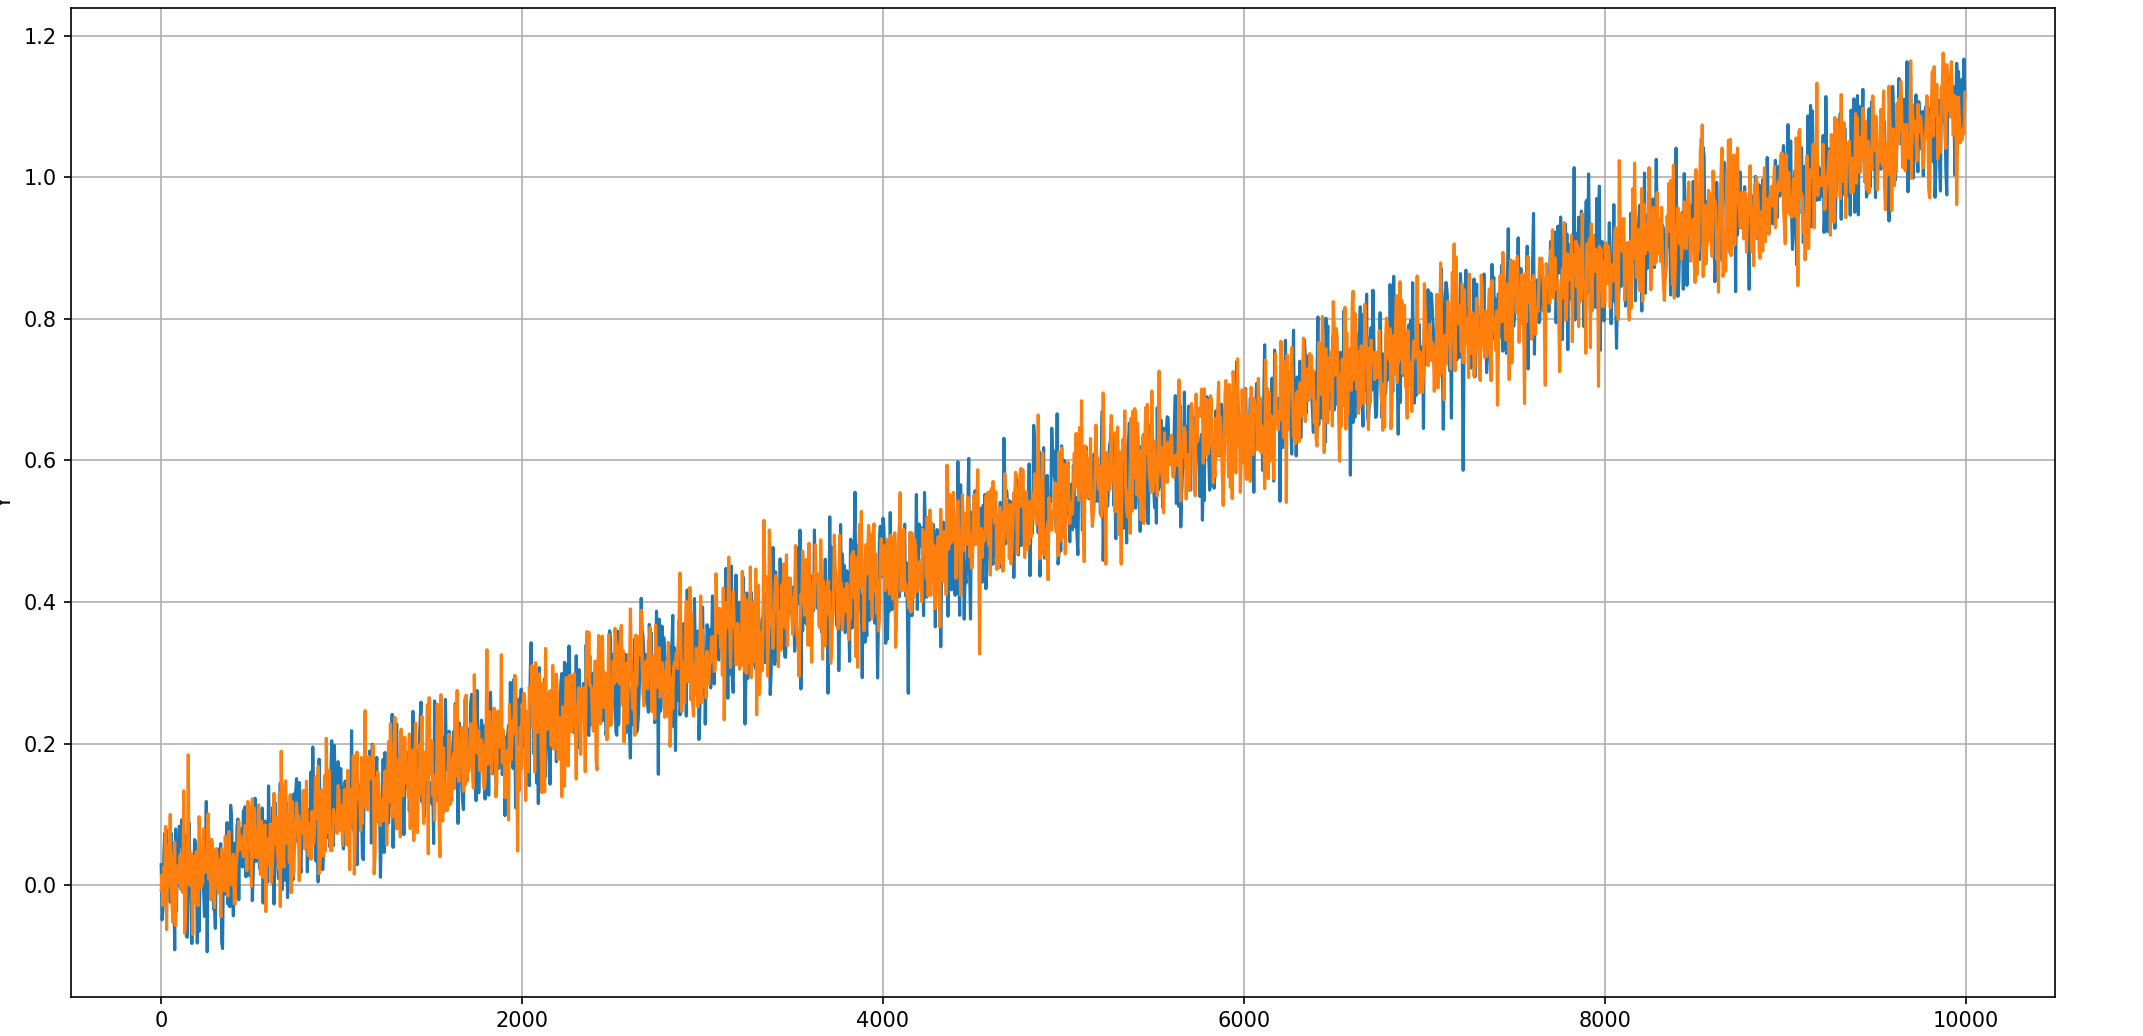
\includegraphics[width=\textwidth]{element/5.png}
    \caption{loop version}
\end{figure}
发现性能基本没有差异,经搜索发现是jvm在优化时会自动消除尾递归,导致性能没有差异.暂时没有找到关闭该优化的方法.
\section{扩展错误处理功能}
\subsection{识别和分类错误}
\textbf{词法错误:}这些错误涉及输入中的非法字符或结构,例如空格、非法字符等。

\textbf{语法错误:}这些错误发生在字符组合违反了语法规则时,例如两个数字之间缺少运算符,或者运算符前缺少操作数。

\subsection{具体实现}
\begin{itemize}
    \item \textbf{空格处理:}通过特定函数\texttt{skipWhitespace()}检查和跳过空格,并标记为词法错误。
    \item \textbf{两个数字之间缺少运算符:}通过状态变量\texttt{expectingOperator}来检测。如果期望一个运算符(例如,读取一个数字后)但是遇到另一个数字,则报告语法错误。
    \item \textbf{运算符前缺少操作数:}同样使用\texttt{expectingOperator}状态。如果期望一个操作数(例如,读取一个运算符后)但是遇到另一个运算符或非法字符,则报告语法错误。
\end{itemize}

\subsection{空格检测}
\begin{figure}[H]
    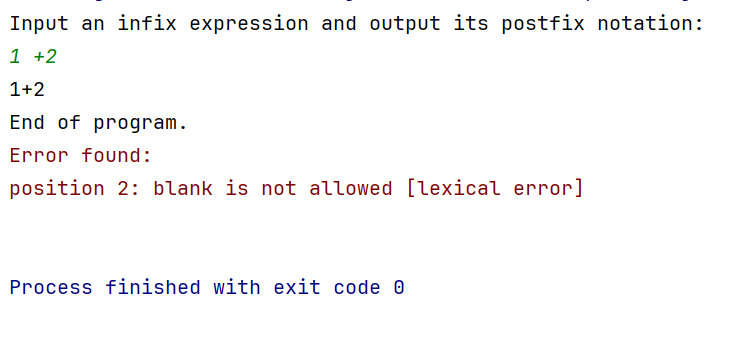
\includegraphics[width=\textwidth]{element/8.png}
    \caption{loop version}
\end{figure}
\subsection{连续运算量错误}
\begin{figure}[H]
    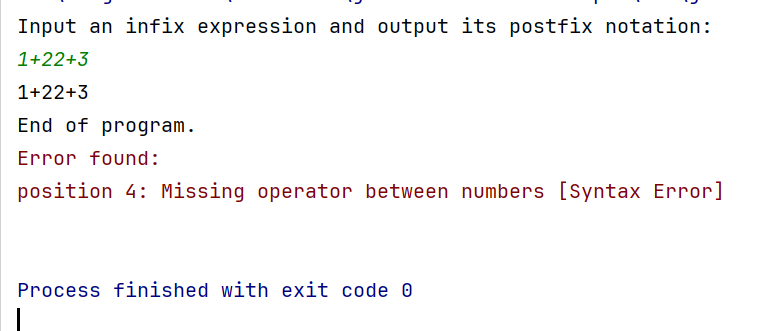
\includegraphics[width=\textwidth]{element/9.png}
    \caption{loop version}
\end{figure}
\subsection{连续运算符错误}
\begin{figure}[H]
    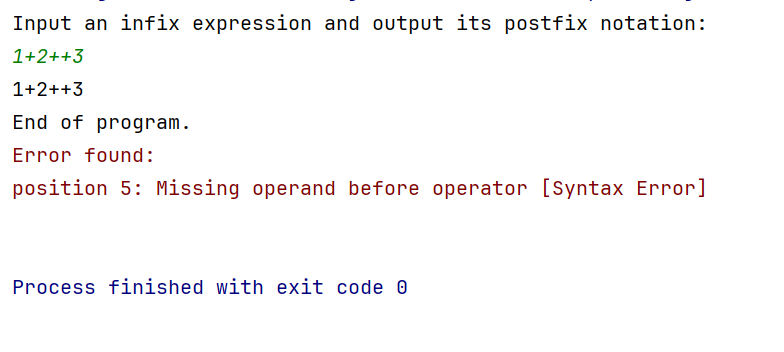
\includegraphics[width=\textwidth]{element/10.png}
    \caption{loop version}
\end{figure}
\subsection{出错恢复与位置}
\begin{itemize}
    \item 在解析器中,使用\texttt{position}变量来跟踪当前处理字符的位置。每当读取一个新字符时,更新\texttt{position}。当报告错误时,使用\texttt{position}来指出错误发生的具体位置
    \item 在遇到错误时,通过\texttt{recover()}函数尝试恢复。此函数的目的是跳过当前的错误点,寻找下一个可能的合法输入点。例如跳过直到找到下一个数字或运算符,从而尝试从新的位置重新开始解析过程。
\end{itemize}


\begin{figure}[H]
    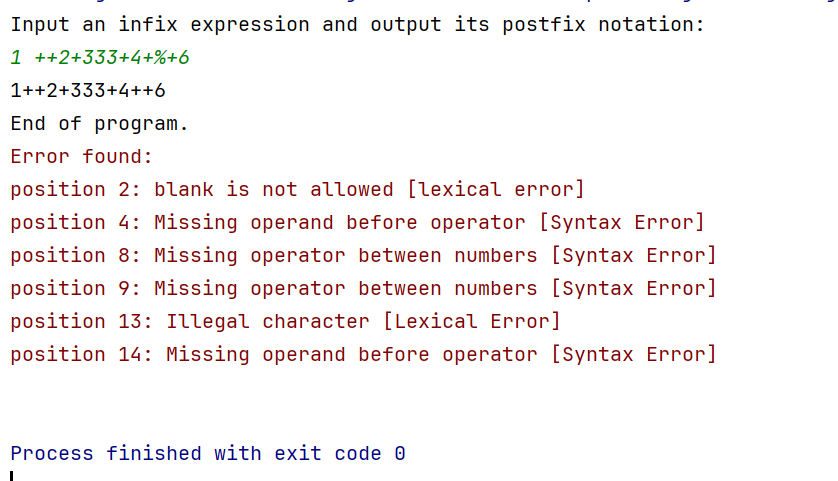
\includegraphics[width=\textwidth]{element/11.png}
    \caption{loop version}
\end{figure}


\end{document}
